\documentclass[12pt]{report}

\usepackage{amsmath}
\usepackage{pgfplots}
\usepgfplotslibrary{units}
\usepackage[russian]{babel}
\usepackage{filecontents}
\usepackage{titlesec, blindtext, color}
\usepackage{listings}
\usepackage{pdfpages}

\usepackage{titlesec, blindtext, color} 
\definecolor{gray75}{gray}{0.75} 
\newcommand{\hsp}{\hspace{20pt}} 

\usepackage{geometry}
\geometry{top=0.5cm}

\lstset{
	language=C++,
	numbers=left,
	breaklines=true, 
	frame=single,
	texcl=true,
	basicstyle=\ttfamily,
	extendedchars=\true
}

\titleformat{\chapter}[hang]{\Huge\bfseries}{\thechapter\hsp\textcolor{gray75}{|}\hsp}{0pt}{\Huge\bfseries}

\begin{document}
	
	
	\begin{titlepage}
		\centering
		{\scshape\LARGE МГТУ им. Баумана \par}
		\vspace{3cm}
		{\scshape\Large Лабораторная работа №6\par}
		\vspace{0.5cm}	
		{\scshape\Large По курсу: "Анализ алгоритмов"\par}
		\vspace{1.5cm}
		{\huge\bfseries Задача коммивояжёра\par}
		\vspace{2cm}
		\Large Работу выполнил: Подвашецкий Дмитрий, ИУ7-54Б\par
		\vspace{0.5cm}
		\LargeПреподаватели:  Волкова Л.Л., Строганов Ю.В.\par
		
		\vfill
		\large \textit {Москва, 2019} \par
	\end{titlepage}
	
	\tableofcontents
	
	\newpage
	\chapter*{Введение}
	\addcontentsline{toc}{chapter}{Введение}
	
	Задача коммивояжёра — одна из самых известных задач комбинаторной оптимизации, заключающаяся в поиске самого выгодного маршрута, проходящего через указанные города хотя бы по одному разу с последующим возвратом в исходный город. В условиях задачи указываются критерий выгодности маршрута (кратчайший, самый дешёвый, совокупный критерий и тому подобное) и соответствующие матрицы расстояний, стоимости и тому подобного. Как правило, указывается, что маршрут должен проходить через каждый город только один раз — в таком случае выбор осуществляется среди гамильтоновых циклов.[4]
	
	Данную задачу можно решить точным методом или же эвристическим. В качестве точного метода будет использован полный перебор, а в качестве эвристического - метод муравьиой колонии.
	
	\textbf{Задачами} данной лабораторной являются:
	\begin{enumerate}
		\item изучение метода полного перебора и метода муравьиной колонии для решения задачи коммивояжёра;
		\item реализация данных двух методов;
		\item экспериментальное подтверждение различий во временнóй эффективности рассматриваемых алгоритмов для различных классов задач;
		\item описание и обоснование полученных результатов в отчете о выполненной лабораторной
		работе, выполненного как расчётно-пояснительная записка к работе.
	\end{enumerate}


	\chapter{Аналитическая часть}
	Задача коммивояжёра относится к классу NP-трудных и не известен алгоритм, который позволет гарантировано её решить за полиномиальное по числу городов N. Однако для небольшого числа городов (N < 15) существует множество способов решения.
	
	В данной лабораторной работе будут исследованы один точный (полный перебо) и один эвристический (муравьиная колония) метод.
	Точные методы позволяют найти наилучший путь, а так же доказать, что найденый путь является таковым.
	В то время как эвристические методы работают существенно быстрее точных, но не гарантируют оптимальности найденого пути.
	
	\textbf{Полный перебор} заключается в перестановки N-1 чисел (при зафиксированном стартовом городе) и поиске пути с минимальной стоимостью (длинной, временем и тд).
	
	\textbf{Метод муравьиной колонии} основан на биологической идеи - принципе существования муравьиной колонии.
	Во время работы данного алгоритма происходит маркировка наиболее удачных путей феромоном.
	
	Работа начинается с размещения муравьёв в вершинах графа (городах), затем начинается движение муравьёв — направление определяется вероятностным методом, на основании формулы вида:

	\begin{equation}
		P_{K, ij} = \begin{cases}
		\dfrac{(\tau_{ij}^\alpha(t))*(\eta_{ij}^\beta)}{\Sigma(\tau_{iq}^\alpha(t))*(\eta_{iq}^\beta)}
		& \textrm{если он не был в городе i}\\ 
		0 & \textrm{иначе}
		\end{cases}
	\end{equation}
	\begin{flushleft}
		$\alpha$, $\beta$ - настроечные параметры
		$\alpha$ + $\beta$  = const
		
		$\tau_{ij}$ - кол-во ферамона на ребре ij
		\begin{equation}
		\eta_{ij} = 1/D_{ij},
		\end{equation}
		{$D_{ij}$} - длина (стоимость) ребра ij
	\end{flushleft}
	
	Дальше с помощью генератора случайных чисел выбирается город, в который мойдет k-тый муравей.
	
	После того, как все муравьи закончили поиск, происходит перерасчет ферамонов по формуле:
	
	\begin{equation}
		\tau_{ij}(t+1) = \tau_{ij}*(1-\rho) + \Sigma\Delta\tau_{k,ij}(t)
	\end{equation}

	$\rho$ - коэф. рассеивания ферамона
	\begin{equation}
	\Delta\tau_{k,ij} = \begin{cases}
	\dfrac{Q}{L_{k}}
	& \textrm{если ij ребро принадлежит маршруту k-го муравья}\\ 
	0 & \textrm{иначе}
	\end{cases}
	\end{equation}
	
	Q - нормировачаная константа
	
	$L_{k}$ - длина пути k-го муравья

	Этот процесс повторяется $T_{max}$ раз. $\alpha$, $\beta$, $T_{max}$ - задаются.[1]
	
	\chapter*{Вывод}
	\addcontentsline{toc}{chapter}{Вывод}
	
	В данном разделе были изучены основные идеи, рассматриваемых в данной лабораторной работе, алгоритмов.
	
	\chapter{Конструкторская часть}
	\section{Схемы алгоритмов}
	\begin{center}
		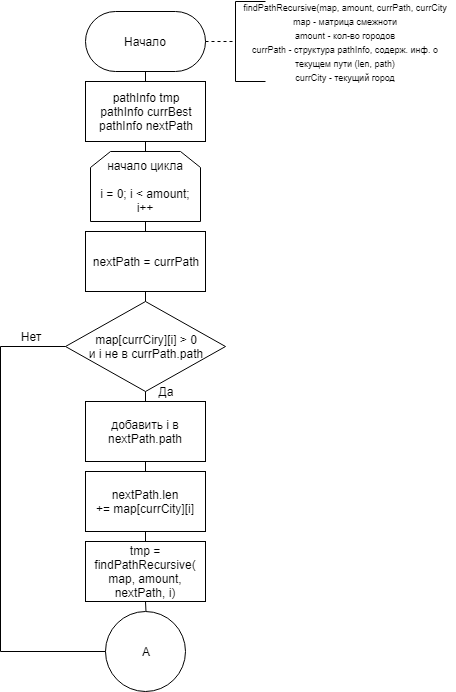
\includegraphics[scale=0.7]{Rec1.png}
		
		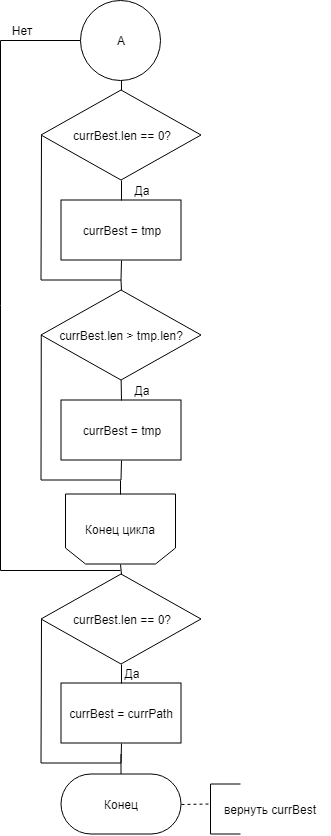
\includegraphics[scale=0.7]{Rec2.png}
		
		Рис. 1. Схема рекурсивной реализации решения задачи коммивояжёра методом полного перебора
		
		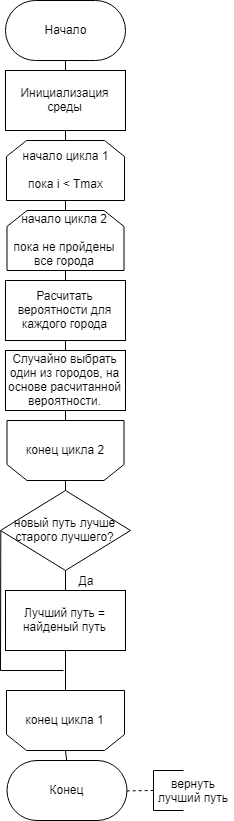
\includegraphics[scale=0.7]{ant.png}
		
		Рис. 2. Схема алгоритма муравьиной колонии
	\end{center}

	\chapter*{Вывод}
	\addcontentsline{toc}{chapter}{Вывод}
	
	В данном разделе были разработаны рассматриваемые в данной лабораторной работе алгоритмы

	\chapter{Технологическая часть}
	\section{Выбор ЯП}
	В качестве языка программирования был выбрал C++, так как он позволяет реализовать задачу максимально комфортно.
	
	\section{Замеры времени}
	Замер времени работы алгоритмов производился при помощи функций clock() из библиотеки time.h.[3]
	
	Также производится усреднение времени работы алгоритмов. Для этого время считается для 5 вызовов, и после делится на 5.
	
	\section{Исследование работы алгоритма муравьиной колонии}

	Так как, при работе данного алгоритма используются случайние числа, то будут использоваться устреденное значение из 5 результатов длины пути найденной колонией при конкретных настроечных параметрах.
	
	\section{Генерация матриц для экспериментов}
	
	Все матрицы будут сгенерированы при помощи программы, написанной на языке Python с ипользованием модуля random и функции randint().[2]
	
	
	\section{Требования к ПО}
	
	\textbf{Требования к вводу:}
	\begin{enumerate}
		\item Имя файла, содержащего матрицу смежности данного графа
	\end{enumerate}
	\textbf{Требования к программе:}
	\begin{enumerate}
		\item Корректный ввод, корректный вывод, программа не должна аварийно завершаться
	\end{enumerate}
	
	\textbf{Требования структуре входного файла:}
	На первой строке написанно одно натуральное число - кол-во вершин.
	Значения в строках должны быть записаны на одной строке. Разделитель - пробел. Конец строки - переход на новую строку.
	
	Пример:
	%\begin{center}
	
		2
		
		0 1
		
		2 0
	%\end{center}
	
	\section{Сведения о модулях программы}
	Программа состоит из:
	\begin{itemize}
		\item main.cpp - главный файл программы
		\item antcolony.cpp - файл с реализациец алгоритма муравьиной колонии (Листинг 3.1.)
		\item recursive.cpp - файл с реализацией алгоритма полного перебора (Листинг 3.2.)
		\item utility.cpp - файл с реализацией доп. функций (т.к. чтение матрица)
	\end{itemize}

	\begin{lstlisting}[label=some-code,caption=Алгоритм муравьиной колонии]
pathInfo runColony(environment &env)
{
	pathInfo curBest;
	
	for (size_t i = 0; i < env.tMax; i++)
	{
		for (size_t j = 0; j < env.cities; j++)
		{
			pathInfo tmp =  runAnt(env, j);
			tmp.len += env.map[tmp.path[0]][tmp.path[tmp.path.size()-1]];
			
			if (tmp.path.size() == env.cities && curBest.len == 0)
				curBest = tmp;
			if (tmp.path.size() == env.cities && curBest.len > tmp.len)
				curBest = tmp;
		}
		
		recalculateTau(env);
	}
	
	return curBest;
}
pathInfo runAnt(environment &env, size_t baseCity)
{
	pathInfo curPath;
	
	while (1)
	{
		std::vector<double> probs;
		double probsDivider = 0;
		if (!isInVector(curPath.path, baseCity))
			curPath.path.push_back(baseCity);
		else
			break;
		
		for (size_t i = 0; i < env.cities; i++)
		{
			if (env.map[baseCity][i] > 0 && !isInVector(curPath.path, i))
			{
				probsDivider += std::pow(env.tau[baseCity][i], env.alpha)*
				std::pow(std::pow(env.map[baseCity][i], -1), env.beta);
			}
		}
		
		for (size_t i = 0; i < env.cities; i++)
		{
			if (isInVector(curPath.path, i) || env.map[baseCity][i] <= 0)
				probs.push_back(0);
			else
				probs.push_back(std::pow(env.tau[baseCity][i], env.alpha)*
				std::pow(std::pow(env.map[baseCity][i], -1), env.beta)/
				probsDivider);
		}
		
		double probsSum = 0;
		for (auto it : probs)
			probsSum += it;
		
		if (probsSum < 0.1)
			break;
		
		double randVal = (double(rand()) / (RAND_MAX)) + 0.000001;
		
		probsSum = 0;
		for (size_t i = 0; i < env.cities; i++)
		{
			probsSum += probs[i];
			if (probsSum >= randVal && !isInVector(curPath.path, i))
			{
				curPath.len += env.map[baseCity][i];
				
				baseCity = i;
				break;
			}
		}
	}
		
	size_t curPathSize = curPath.path.size();
	if (curPathSize == env.cities)
	{
		double dTau = env.Q / curPath.len;
		for (size_t i = 0; i < curPathSize - 1; i++)
		{
			env.dTau[curPath.path[i]][curPath.path[i+1]] += dTau;
			env.dTau[curPath.path[i+1]][curPath.path[i]] += dTau;
		}
	}
	
	return curPath;
}
void recalculateTau(environment &env)
{
	for (size_t i = 0; i < env.cities; i++)
	{
		for (size_t j = 0; j < env.cities; j++)
		{
			env.tau[i][j] = env.tau[i][j]*(1 - env.ro) + env.dTau[i][j];
			env.dTau[i][j] = 0;
		}
	}
}

	\end{lstlisting}
	
	\begin{lstlisting}[label=some-code,caption=Алгоритм полного перебора]
pathInfo findPathRecursiveForAll(const MtrInt &map, const size_t amount)
{
	pathInfo best;
	pathInfo tmp;
	
	for (size_t i = 0; i < amount; i++)
	{
		pathInfo def;
		def.path.push_back(i);
		tmp = findPathRecursive(map, amount, def, i);
		tmp.len += map[tmp.path[0]][tmp.path[tmp.path.size()-1]];
		
		if (best.len == 0)
			best = tmp;
		if (best.len > tmp.len)
			best = tmp;
	}
	
	return best;
}
pathInfo findPathRecursive(const MtrInt &map,const size_t amount, pathInfo currPath, size_t currCity)
{
	pathInfo tmp;
	pathInfo currBest;
	pathInfo nextPath;
	
	for (size_t i = 0; i < amount; i++)
	{
		nextPath = currPath;
		if (map[currCity][i] > 0 && !isInVector(currPath.path, i))
		{
			nextPath.path.push_back(i);
			nextPath.len += map[currCity][i];
			tmp = findPathRecursive(map, amount, nextPath, i);
			
			if (currBest.len == 0)
				currBest = tmp;
			if (currBest.len > tmp.len)
				currBest = tmp;
		}
	}
	
	if (currBest.len == 0)
		currBest = currPath;
	
	return currBest;
}
	\end{lstlisting}
	
	\chapter*{Вывод}
	\addcontentsline{toc}{chapter}{Вывод}
	
	В данном разделе были реализованны рассматриваемые алгоритмы.
	
	\chapter{Экспериментальная часть}
	
	На работу метода муравьиной колонии влияют 3 параметра: $\alpha$ - коэффициент стадности, т.е. то, насколько важным будет являться ферамон при выборе следующего города, $\beta$ - коэффициент жадности, т.е. то, насколько важным будет являтся длина ребра и $T_{max}$ - сколько итераций совершит алгоритм.
	
	\begin{center}
		Параметр $\alpha$ будет меняться в пределе [0, 1] с шагом 0.1. $\beta$ будет вычисляться как 1 - $\alpha$.
		$T_{max}$ будет менять в пределе [10, 130] c шагом 20.
	\end{center}
	
	В данном разделе будут выделены 2 класса задач, и подобраны оптимальные значения настроечных параметров для каждого из них.
	
	Классы задач:
	\begin{enumerate}
		\item граф, в котором длины ребер одного порядка;
		\item граф, в котором длины отличаются на нескольно порядков.
	\end{enumerate}
	
	\section{Анализ настроечных параметров}
	\subsection{Первый класс задач}
	
	Для первого класса задач была сгенерирована матрица:
	\begin{center}
		$
		\begin{pmatrix}
			0 & 38 & 51 & 36 & 66 & 73 & 44 & 80 \\ 
			38 & 0 & 72 & 59 & 72 & 35 & 45 & 58 \\ 
			51 &  72 & 0 & 59 & 51 & 44 & 63 & 44 \\
			36 & 59 & 59 & 0 & 44 & 36 & 76 & 53 \\
			66 & 72 & 51 & 44 & 0 & 67 & 54 & 56 \\
			73 & 35 & 44 & 36 & 67 & 0 & 53 & 30 \\
			44 & 45 & 63 & 76 & 54 & 53 & 0 & 30 \\
			80 & 58 & 44 & 53 & 56 & 30 & 30 & 0 
		\end{pmatrix}
		$
	\end{center}

	В этой матрице все длины ребер находятся в промежутке [30, 80] усл. ед..
	~\\
	~\\
	Результаты полного перебора: Длина - 318, Время - 0.31 (с).

	\begin{minipage}{0.5\textwidth}
			\begin{center}
				Таблица 1.1.
				
				\begin{tabular}{|c c c c c|}
					\hline
					$\alpha$ & $\beta$ & $T_{max}$ & Len & Time (c) \\ [0.5ex]
					0 & 1 & 10 & 344 & 0.0042 \\ 
					\hline 
					0 & 1 & 30 & 320 & 0.0134 \\ 
					\hline 
					0 & 1 & 50 & 322 & 0.0162 \\ 
					\hline 
					0 & 1 & 70 & 318 & 0.0228 \\ 
					\hline 
					0 & 1 & 90 & 321 & 0.0288 \\ 
					\hline 
					0 & 1 & 110 & 318 & 0.0354 \\ 
					\hline 
					0 & 1 & 130 & 319 & 0.0422 \\ 
					\hline 
				\end{tabular}
			
				Таблица 1.2.
				
				\begin{tabular}{|c c c c c|}
					\hline
					$\alpha$ & $\beta$ & $T_{max}$ & Len & Time (c) \\ [0.5ex]
					0.1 & 0.9 & 10 & 322 & 0.004 \\ 
					\hline 
					0.1 & 0.9 & 30 & 326 & 0.0118 \\ 
					\hline 
					0.1 & 0.9 & 50 & 321 & 0.0196 \\ 
					\hline 
					0.1 & 0.9 & 70 & 319 & 0.028 \\ 
					\hline 
					0.1 & 0.9 & 90 & 318 & 0.0348 \\ 
					\hline 
					0.1 & 0.9 & 110 & 318 & 0.043 \\ 
					\hline 
					0.1 & 0.9 & 130 & 318 & 0.0506 \\ 
					\hline 
				\end{tabular}
			
				Таблица 1.3.
				
				\begin{tabular}{|c c c c c|}
					\hline
					$\alpha$ & $\beta$ & $T_{max}$ & Len & Time (c) \\ [0.5ex]
					0.2 & 0.8 & 10 & 327 & 0.0036 \\ 
					\hline 
					0.2 & 0.8 & 30 & 326 & 0.0118 \\ 
					\hline 
					0.2 & 0.8 & 50 & 321 & 0.02 \\ 
					\hline 
					0.2 & 0.8 & 70 & 319 & 0.0276 \\ 
					\hline 
					0.2 & 0.8 & 90 & 320 & 0.0354 \\ 
					\hline 
					0.2 & 0.8 & 110 & 319 & 0.043 \\ 
					\hline 
					0.2 & 0.8 & 130 & 320 & 0.0508 \\ 
					\hline 
				\end{tabular}
			
				Таблица 1.4.
				
				\begin{tabular}{|c c c c c|}
					\hline
					$\alpha$ & $\beta$ & $T_{max}$ & Len & Time (c) \\ [0.5ex]
					0.3 & 0.7 & 10 & 338 & 0.0042 \\ 
					\hline 
					0.3 & 0.7 & 30 & 322 & 0.0118 \\ 
					\hline 
					0.3 & 0.7 & 50 & 324 & 0.0196 \\ 
					\hline 
					0.3 & 0.7 & 70 & 319 & 0.0276 \\ 
					\hline 
					0.3 & 0.7 & 90 & 318 & 0.0352 \\ 
					\hline 
					0.3 & 0.7 & 110 & 320 & 0.0426 \\ 
					\hline 
					0.3 & 0.7 & 130 & 320 & 0.0516 \\ 
					\hline 
				\end{tabular}
				
			\end{center}
	\end{minipage}
	\hfill
	\begin{minipage}{0.5\textwidth}
		\begin{center}
			Таблица 1.5.
			
			\begin{tabular}{|c c c c c|}
				\hline
				$\alpha$ & $\beta$ & $T_{max}$ & Len & Time (c) \\ [0.5ex]
				0.4 & 0.6 & 10 & 330 & 0.004 \\ 
				\hline 
				0.4 & 0.6 & 30 & 322 & 0.0122 \\ 
				\hline 
				0.4 & 0.6 & 50 & 322 & 0.0196 \\ 
				\hline 
				0.4 & 0.6 & 70 & 320 & 0.0276 \\ 
				\hline 
				0.4 & 0.6 & 90 & 319 & 0.0352 \\ 
				\hline 
				0.4 & 0.6 & 110 & 318 & 0.043 \\ 
				\hline 
				0.4 & 0.6 & 130 & 320 & 0.0512 \\ 
				\hline 
			\end{tabular}
			
			Таблица 1.6.
			
			\begin{tabular}{|c c c c c|}
				\hline
				$\alpha$ & $\beta$ & $T_{max}$ & Len & Time (c) \\ [0.5ex]
				0.5 & 0.5 & 10 & 338 & 0.0032 \\ 
				\hline 
				0.5 & 0.5 & 30 & 325 & 0.0096 \\ 
				\hline 
				0.5 & 0.5 & 50 & 318 & 0.0172 \\ 
				\hline 
				0.5 & 0.5 & 70 & 321 & 0.0238 \\ 
				\hline 
				0.5 & 0.5 & 90 & 320 & 0.03 \\ 
				\hline 
				0.5 & 0.5 & 110 & 319 & 0.0364 \\ 
				\hline 
				0.5 & 0.5 & 130 & 318 & 0.043 \\ 
				\hline 
			\end{tabular}
		
			Таблица 1.7.
			
			\begin{tabular}{|c c c c c|}
				\hline
				$\alpha$ & $\beta$ & $T_{max}$ & Len & Time (c) \\ [0.5ex]
				0.6 & 0.4 & 10 & 328 & 0.0038 \\ 
				\hline 
				0.6 & 0.4 & 30 & 327 & 0.0118 \\ 
				\hline 
				0.6 & 0.4 & 50 & 319 & 0.0194 \\ 
				\hline 
				0.6 & 0.4 & 70 & 318 & 0.0278 \\ 
				\hline 
				0.6 & 0.4 & 90 & 318 & 0.0346 \\ 
				\hline 
				0.6 & 0.4 & 110 & 320 & 0.0434 \\ 
				\hline 
				0.6 & 0.4 & 130 & 318 & 0.0504 \\ 
				\hline 
			\end{tabular}
		
			Таблица 1.8.
		
			\begin{tabular}{|c c c c c|}
				\hline
				$\alpha$ & $\beta$ & $T_{max}$ & Len & Time (c) \\ [0.5ex]
				0.7 & 0.3 & 10 & 328 & 0.004 \\ 
				\hline 
				0.7 & 0.3 & 30 & 322 & 0.012 \\ 
				\hline 
				0.7 & 0.3 & 50 & 319 & 0.0192 \\ 
				\hline 
				0.7 & 0.3 & 70 & 320 & 0.0272 \\ 
				\hline 
				0.7 & 0.3 & 90 & 320 & 0.035 \\ 
				\hline 
				0.7 & 0.3 & 110 & 318 & 0.0428 \\ 
				\hline 
				0.7 & 0.3 & 130 & 318 & 0.0502 \\ 
				\hline 
			\end{tabular}
		
			
		
		\end{center}
	\end{minipage}

	\newpage

	\begin{minipage}{0.5\textwidth}
		\begin{center}
			Таблица 1.9.
			
			\begin{tabular}{|c c c c c|}
				\hline
				$\alpha$ & $\beta$ & $T_{max}$ & Len & Time (c) \\ [0.5ex]
				0.9 & 0.1 & 10 & 339 & 0.004 \\ 
				\hline 
				0.9 & 0.1 & 30 & 332 & 0.0118 \\ 
				\hline 
				0.9 & 0.1 & 50 & 324 & 0.0198 \\ 
				\hline 
				0.9 & 0.1 & 70 & 319 & 0.0276 \\ 
				\hline 
				0.9 & 0.1 & 90 & 318 & 0.0352 \\ 
				\hline 
				0.9 & 0.1 & 110 & 319 & 0.044 \\ 
				\hline 
				0.9 & 0.1 & 130 & 319 & 0.0516 \\ 
				\hline 
			\end{tabular}
		\end{center}
	\end{minipage}
	\hfill
	\begin{minipage}{0.5\textwidth}
		\begin{center}
			Таблица 1.10.
			
			\begin{tabular}{|c c c c c|}
				\hline
				$\alpha$ & $\beta$ & $T_{max}$ & Len & Time (c) \\ [0.5ex]
				1 & 0 & 10 & 348 & 0.0032 \\ 
				\hline 
				1 & 0 & 30 & 327 & 0.0094 \\ 
				\hline 
				1 & 0 & 50 & 327 & 0.0164 \\ 
				\hline 
				1 & 0 & 70 & 322 & 0.0228 \\ 
				\hline 
				1 & 0 & 90 & 320 & 0.029 \\ 
				\hline 
				1 & 0 & 110 & 322 & 0.0358 \\ 
				\hline 
				1 & 0 & 130 & 325 & 0.0422 \\ 
				\hline 
			\end{tabular}
		\end{center}
	\end{minipage}

	\begin{center}
		Таблица 1.11.
		
		\begin{tabular}{|c c c c c|}
			\hline
			$\alpha$ & $\beta$ & $T_{max}$ & Len & Time (c) \\ [0.5ex]
			0.8 & 0.2 & 10 & 343 & 0.004 \\ 
			\hline 
			0.8 & 0.2 & 30 & 330 & 0.0116 \\ 
			\hline 
			0.8 & 0.2 & 50 & 323 & 0.0196 \\ 
			\hline 
			0.8 & 0.2 & 70 & 318 & 0.0272 \\ 
			\hline 
			0.8 & 0.2 & 90 & 319 & 0.0354 \\ 
			\hline 
			0.8 & 0.2 & 110 & 319 & 0.0424 \\ 
			\hline 
			0.8 & 0.2 & 130 & 321 & 0.051 \\ 
			\hline 
		\end{tabular}
	\end{center}
		
	Анализируя Таблицы 1.1. - 1.11. можно сделать вывод, что для данного класса задач наиболее подходит конфигурация ($\alpha$ = 0.6, $\beta$ = 0.4) из Таблицы 1.7., так как уже при 50 итерациях удается получить наиболее удачный результат за 0.0278 секунды, что в 11 раз быстрее полного перебора.
	
	
	\subsection{Второй класс задач}
	
	Для второго класса задач была сгенерирована матрица:
	\begin{center}
		$
		\begin{pmatrix}
		0 & 43 & 531 & 406 & 4 & 124 & 234 & 117 \\
		43 & 0 & 112 & 24 & 416 & 240 & 86 & 229 \\
		531 & 112 & 0 & 370 & 540 & 389 & 583 & 38 \\
		406 & 24 & 370 & 0 & 337 & 220 & 369 & 129 \\
		4 & 416 & 540 & 337 & 0 & 543 & 77 & 208 \\
		124 & 240 & 389 & 220 & 543 & 0 & 306 & 154 \\ 
		234 & 86 & 583 & 369 & 77 & 306 & 0 & 368 \\
		117 & 229 & 38 & 129 & 208 & 154 & 368 & 0 \\
		\end{pmatrix}
		$
	\end{center}                 

	В данной матрице все длины ребер находятся в промежутке [1, 600] усл. ед..
	~\\
	~\\
	Результат полного перебора: Длина - 318, Время - 0.28 (с).
	
	\newpage
	
	\begin{minipage}{0.5\textwidth}
		\begin{center}
			Таблица 2.1.
			
			\begin{tabular}{|c c c c c|}
				\hline
				$\alpha$ & $\beta$ & $T_{max}$ & Len & Time (c) \\ [0.5ex]
				0 & 1 & 10 & 856 & 0.0034 \\ 
				\hline 
				0 & 1 & 30 & 806 & 0.01 \\ 
				\hline 
				0 & 1 & 50 & 790 & 0.017 \\ 
				\hline 
				0 & 1 & 70 & 790 & 0.023 \\ 
				\hline 
				0 & 1 & 90 & 790 & 0.0312 \\ 
				\hline 
				0 & 1 & 110 & 790 & 0.0358 \\ 
				\hline 
				0 & 1 & 130 & 790 & 0.0424 \\ 
				\hline 
			\end{tabular}
			
			Таблица 2.2.
			
			\begin{tabular}{|c c c c c|}
				\hline
				$\alpha$ & $\beta$ & $T_{max}$ & Len & Time (c) \\ [0.5ex]
				0.1 & 0.9 & 10 & 822 & 0.004 \\ 
				\hline 
				0.1 & 0.9 & 30 & 790 & 0.0118 \\ 
				\hline 
				0.1 & 0.9 & 50 & 790 & 0.0198 \\ 
				\hline 
				0.1 & 0.9 & 70 & 790 & 0.028 \\ 
				\hline 
				0.1 & 0.9 & 90 & 790 & 0.0352 \\ 
				\hline 
				0.1 & 0.9 & 110 & 790 & 0.0436 \\ 
				\hline 
				0.1 & 0.9 & 130 & 790 & 0.0524 \\ 
				\hline 
			\end{tabular}
			
			Таблица 2.3.
			
			\begin{tabular}{|c c c c c|}
				\hline
				$\alpha$ & $\beta$ & $T_{max}$ & Len & Time (c) \\ [0.5ex]
				0.2 & 0.8 & 10 & 845 & 0.004 \\ 
				\hline 
				0.2 & 0.8 & 30 & 790 & 0.0118 \\ 
				\hline 
				0.2 & 0.8 & 50 & 790 & 0.0206 \\ 
				\hline 
				0.2 & 0.8 & 70 & 790 & 0.0296 \\ 
				\hline 
				0.2 & 0.8 & 90 & 790 & 0.0358 \\ 
				\hline 
				0.2 & 0.8 & 110 & 790 & 0.0434 \\ 
				\hline 
				0.2 & 0.8 & 130 & 790 & 0.0532 \\ 
				\hline 
			\end{tabular}
			
			Таблица 2.4.
			
			\begin{tabular}{|c c c c c|}
				\hline
				$\alpha$ & $\beta$ & $T_{max}$ & Len & Time (c) \\ [0.5ex]
				0.3 & 0.7 & 10 & 806 & 0.004 \\ 
				\hline 
				0.3 & 0.7 & 30 & 790 & 0.012 \\ 
				\hline 
				0.3 & 0.7 & 50 & 790 & 0.0206 \\ 
				\hline 
				0.3 & 0.7 & 70 & 790 & 0.0274 \\ 
				\hline 
				0.3 & 0.7 & 90 & 790 & 0.0368 \\ 
				\hline 
				0.3 & 0.7 & 110 & 790 & 0.0436 \\ 
				\hline 
				0.3 & 0.7 & 130 & 790 & 0.0518 \\ 
				\hline 
			\end{tabular}
			
		\end{center}
	\end{minipage}
	\hfill
	\begin{minipage}{0.5\textwidth}
		\begin{center}
			Таблица 2.5.
			
		\begin{tabular}{|c c c c c|}
			\hline
			$\alpha$ & $\beta$ & $T_{max}$ & Len & Time (c) \\ [0.5ex]
			0.4 & 0.6 & 10 & 822 & 0.0036 \\ 
			\hline 
			0.4 & 0.6 & 30 & 790 & 0.0118 \\ 
			\hline 
			0.4 & 0.6 & 50 & 790 & 0.0202 \\ 
			\hline 
			0.4 & 0.6 & 70 & 790 & 0.0284 \\ 
			\hline 
			0.4 & 0.6 & 90 & 790 & 0.0366 \\ 
			\hline 
			0.4 & 0.6 & 110 & 790 & 0.0454 \\ 
			\hline 
			0.4 & 0.6 & 130 & 790 & 0.0506 \\ 
			\hline 
		\end{tabular}
			
			Таблица 2.6.
			
			\begin{tabular}{|c c c c c|}
				\hline
				$\alpha$ & $\beta$ & $T_{max}$ & Len & Time (c) \\ [0.5ex]
				0.5 & 0.5 & 10 & 839 & 0.0032 \\ 
				\hline 
				0.5 & 0.5 & 30 & 790 & 0.0104 \\ 
				\hline 
				0.5 & 0.5 & 50 & 790 & 0.0166 \\ 
				\hline 
				0.5 & 0.5 & 70 & 790 & 0.0232 \\ 
				\hline 
				0.5 & 0.5 & 90 & 790 & 0.0306 \\ 
				\hline 
				0.5 & 0.5 & 110 & 790 & 0.0372 \\ 
				\hline 
				0.5 & 0.5 & 130 & 790 & 0.0446 \\ 
				\hline 
			\end{tabular}
			
			Таблица 2.7.
			
			\begin{tabular}{|c c c c c|}
				\hline
				$\alpha$ & $\beta$ & $T_{max}$ & Len & Time (c) \\ [0.5ex]
				0.6 & 0.4 & 10 & 871 & 0.004 \\ 
				\hline 
				0.6 & 0.4 & 30 & 790 & 0.012 \\ 
				\hline 
				0.6 & 0.4 & 50 & 790 & 0.0204 \\ 
				\hline 
				0.6 & 0.4 & 70 & 790 & 0.027 \\ 
				\hline 
				0.6 & 0.4 & 90 & 790 & 0.0356 \\ 
				\hline 
				0.6 & 0.4 & 110 & 790 & 0.0442 \\ 
				\hline 
				0.6 & 0.4 & 130 & 790 & 0.0516 \\ 
				\hline 
			\end{tabular}
			
			Таблица 2.8.
			
			\begin{tabular}{|c c c c c|}
				\hline
				$\alpha$ & $\beta$ & $T_{max}$ & Len & Time (c) \\ [0.5ex]
				0.7 & 0.3 & 10 & 839 & 0.004 \\ 
				\hline 
				0.7 & 0.3 & 30 & 822 & 0.0128 \\ 
				\hline 
				0.7 & 0.3 & 50 & 790 & 0.0196 \\ 
				\hline 
				0.7 & 0.3 & 70 & 790 & 0.027 \\ 
				\hline 
				0.7 & 0.3 & 90 & 790 & 0.0362 \\ 
				\hline 
				0.7 & 0.3 & 110 & 790 & 0.0436 \\ 
				\hline 
				0.7 & 0.3 & 130 & 790 & 0.053 \\ 
				\hline 
			\end{tabular}
			
			
			
		\end{center}
	\end{minipage}
	
	\newpage
	
	\begin{minipage}{0.5\textwidth}
		\begin{center}
			Таблица 2.9.
			
			\begin{tabular}{|c c c c c|}
				\hline
				$\alpha$ & $\beta$ & $T_{max}$ & Len & Time (c) \\ [0.5ex]
				0.9 & 0.1 & 10 & 919 & 0.004 \\ 
				\hline 
				0.9 & 0.1 & 30 & 834 & 0.012 \\ 
				\hline 
				0.9 & 0.1 & 50 & 823 & 0.0198 \\ 
				\hline 
				0.9 & 0.1 & 70 & 790 & 0.0278 \\ 
				\hline 
				0.9 & 0.1 & 90 & 790 & 0.036 \\ 
				\hline 
				0.9 & 0.1 & 110 & 790 & 0.044 \\ 
				\hline 
				0.9 & 0.1 & 130 & 790 & 0.0516 \\ 
				\hline 
			\end{tabular}
		\end{center}
	\end{minipage}
	\hfill
	\begin{minipage}{0.5\textwidth}
		\begin{center}
			Таблица 2.10.
			
			\begin{tabular}{|c c c c c|}
				\hline
				$\alpha$ & $\beta$ & $T_{max}$ & Len & Time (c) \\ [0.5ex]
				1 & 0 & 10 & 1088 & 0.0034 \\ 
				\hline 
				1 & 0 & 30 & 914 & 0.0098 \\ 
				\hline 
				1 & 0 & 50 & 885 & 0.0174 \\ 
				\hline 
				1 & 0 & 70 & 806 & 0.0228 \\ 
				\hline 
				1 & 0 & 90 & 807 & 0.0294 \\ 
				\hline 
				1 & 0 & 110 & 790 & 0.0374 \\ 
				\hline 
				1 & 0 & 130 & 790 & 0.0428 \\ 
				\hline 
			\end{tabular}
		\end{center}
	\end{minipage}
	
	\begin{center}
		Таблица 2.11.
		
		\begin{tabular}{|c c c c c|}
			\hline
			$\alpha$ & $\beta$ & $T_{max}$ & Len & Time (c) \\ [0.5ex]
			0.8 & 0.2 & 10 & 950 & 0.0042 \\ 
			\hline 
			0.8 & 0.2 & 30 & 806 & 0.0118 \\ 
			\hline 
			0.8 & 0.2 & 50 & 790 & 0.02 \\ 
			\hline 
			0.8 & 0.2 & 70 & 790 & 0.0284 \\ 
			\hline 
			0.8 & 0.2 & 90 & 790 & 0.0356 \\ 
			\hline 
			0.8 & 0.2 & 110 & 790 & 0.0438 \\ 
			\hline 
			0.8 & 0.2 & 130 & 790 & 0.0506 \\ 
			\hline 
		\end{tabular}
	\end{center}
			
	Анализируя Таблицы 2.1. - 2.11. можно сделать вывод, что для данного класса задач наиболее подходит конфигурация ($\alpha$ = 0.3, $\beta$ = 0.7) из Таблицы 2.4., так как уже при 30 итерациях удается получить наиболее удачный результат за 0.012 секунды, что в 23, раз быстрее полного перебора.
	
	\chapter*{Вывод}
	\addcontentsline{toc}{chapter}{Вывод}
	
	Анализируя данные, полученные в этом разделе, можно сделать вывод, что для задач, в которых длины ребер примерно одинаковы (первый класс задач) предпочтительнее, когда коэффициент стадности превышает коэффициент жадности, т.е. лучше ориентироваться на длине ребер.
	Иначе, если длины ребер сильно разнятся (второй класс задач) предпочтительнее обратная ситуация, при которой муравьи ориентируются на кол-во феромоном на том или ином ребре.
	
	Для первого случая наиболее удачной была выбрана конфигурация ($\alpha$ = 0.6, $\beta$ = 0.4).
	Для второго случая наиболее удачной была выбрана конфигурация ($\alpha$ = 0.3, $\beta$ = 0.7).
	
	
	\chapter*{Заключение}
	\addcontentsline{toc}{chapter}{Заключение}
	
	При написании данной лабораторной работы были изучены и реализованы точный метод решения задачи коммивояжёра - полный перебор, а так же эвристический метод муравьиной колонии.
	
	Были выделены два класса задач и проведены исследования различных конфигураций настроечных параметров для каждого из классов.
	
	Первым классом задач были выбраны такие, где длины ребер в графе различаются незначительно.
	Оптимальной конфигурацией было выбрано - ($\alpha$ = 0.6, $\beta$ = 0.4).
	
	Вторым классом задач были выбраны такие, где длины ребер в графе различаются значительно.
	Оптимальной конфигурацией было выбрано - ($\alpha$ = 0.3, $\beta$ = 0.7).
	
	\chapter*{Список литературы}
	\addcontentsline{toc}{chapter}{Список литературы}
	\begin{enumerate}
		\item Муравьиный алгоритм. [Электронный ресурс] Режим доступа: http://smart-blog.net/post/2359 Последння дата обращения: 03.12.2019
		\item random — Generate pseudo-random numbers. [Электронный ресурс] Режим доступа: https://docs.python.org/3/library/random.html Последння дата обращения: 03.12.2019
		\item Заголовочный файл ctime (time.h). [Электронный ресурс] Режим доступа: http://cppstudio.com/cat/309/326/ Последння дата обращения: 03.12.2019
		\item Задача коммивояжёра. [Электронный ресурс] Режим доступа: http://synset.com Последння дата обращения: 03.12.2019
	\end{enumerate}
	
		
	
	
		
	
	
	
	
	
	
	
	
	
	
	
	
	
	
	
	
	
	
	
	
	
	
	
	
	
	
	
	
	
	
	
	
	
\end{document}